\documentclass{article}
\usepackage{amsmath, sfmath, multicol, tkz-euclide, array, enumerate, tcolorbox, tabularray}
\renewcommand{\familydefault}{\sfdefault}
\setlength{\parindent}{0cm}
\pagestyle{empty}
\usepackage[left=1in, top=0.5in, right=1in, bottom=0.5in]{geometry}
\tikzset{>=stealth}
\tcbset{colback=white}

\newcounter{example}[section]
\newenvironment{example}[1][]{\refstepcounter{example}\par\medskip
   {\color{red}\textbf{Example~\theexample. #1}}}{\medskip}

\begin{document}

\section*{Triangle Congruence by SSS and SAS}

\begin{tcolorbox}[colframe=orange!70!white, coltitle=black, title=\textbf{Today I Can}]
\begin{enumerate}
    \item Prove triangles congruent by SSS and SAS shortcuts.
\end{enumerate}
\end{tcolorbox}

In this section, we will learn some shortcuts to proving 2 triangles congruent. \newline

Instead of needing to prove \underline{all} corresponding angle and side pairs congruent, we only need to establish
\begin{itemize}
    \item Three pairs of congruent, corresponding sides --OR--
    \item Two pairs of congruent, corresponding sides and the angles between them congruent
\end{itemize}

\bigskip 

\begin{tcolorbox}[colframe=black!20!white, opacitybacktitle=0.1, coltitle=black, title=\textbf{Side-Side-Side (SSS) Shortcut}]
If 3 sides of one triangle are congruent to 3 sides of another, then the triangles are congruent.
\newline

\begin{minipage}{0.3\textwidth}
\begin{itemize}
    \item $\triangle ABC \cong \triangle DEF$
\end{itemize}
\end{minipage}
\begin{minipage}{0.6\textwidth}
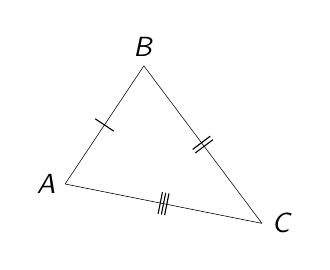
\begin{tikzpicture}
\tkzDefPoints{0/0/A, 1/1.5/B, 2.5/-0.5/C}
\tkzDrawPolygon(A,B,C)
\tkzLabelPoints[left](A)
\tkzLabelPoints[above](B)
\tkzLabelPoints[right](C)
\tkzMarkSegment[mark = |](A,B)
\tkzMarkSegment[mark = ||](B,C)
\tkzMarkSegment[mark = |||](A,C)
\end{tikzpicture}
\hspace{0.25in}
\begin{tikzpicture}
\tkzDefPoints{0/0/D, 1/1.5/E, 2.5/-0.5/F}
\tkzDrawPolygon(D,E,F)
\tkzLabelPoints[left](D)
\tkzLabelPoints[above](E)
\tkzLabelPoints[right](F)
\tkzMarkSegment[mark = |](D,E)
\tkzMarkSegment[mark = ||](E,F)
\tkzMarkSegment[mark = |||](D,F)
\end{tikzpicture}
\end{minipage}
\end{tcolorbox}

\begin{example}
\textbf{Given:} $\overline{LM} \cong \overline{MP}$ and $\overline{LP} \cong \overline{NM}$
\qquad
\textbf{Prove:} $\triangle LMN \cong \triangle NPL$ \newline\\
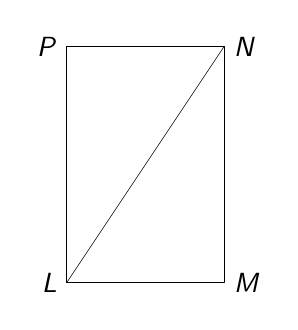
\begin{tikzpicture}
    \tkzDefPoints{0/0/L, 2/0/M, 2/3/N, 0/3/P}
    \tkzDrawPolygon(L,M,N,P)
    \tkzLabelPoints[right](M,N)
    \tkzLabelPoints[left](L,P)
    \tkzDrawSegment(L,N)
\end{tikzpicture}
\end{example}

\vfill 

\begin{example}
\textbf{Given:} $\overline{BC} \cong \overline{BF}$ and $\overline{CD} \cong \overline{FD}$
\qquad
\textbf{Prove:} $\triangle BCD \cong \triangle BFD$
\newline

\begin{tikzpicture}
    \tkzDefPoints{0/0/B, 3.25/0/D, 1/1.25/C, 1/-1.25/F}
    \tkzDrawPolygon(B,C,D,F)
    \tkzDrawSegment(B,D)
    \tkzLabelPoints[left](B)
    \tkzLabelPoints[above](C)
    \tkzLabelPoints[right](D)
    \tkzLabelPoints[below](F)
\end{tikzpicture}
\end{example}

\vfill 
\newpage 

\begin{example}
Prove $\triangle ABC \cong \triangle DEF$ if
\newline

$A(1, \, -1), \, B(2, \, 2), \, C(6, \, 2) \hspace{0.25in} D(-1, \, 1), \, E(-2, \, -2), \, F(-6, \, -2)$ \newline

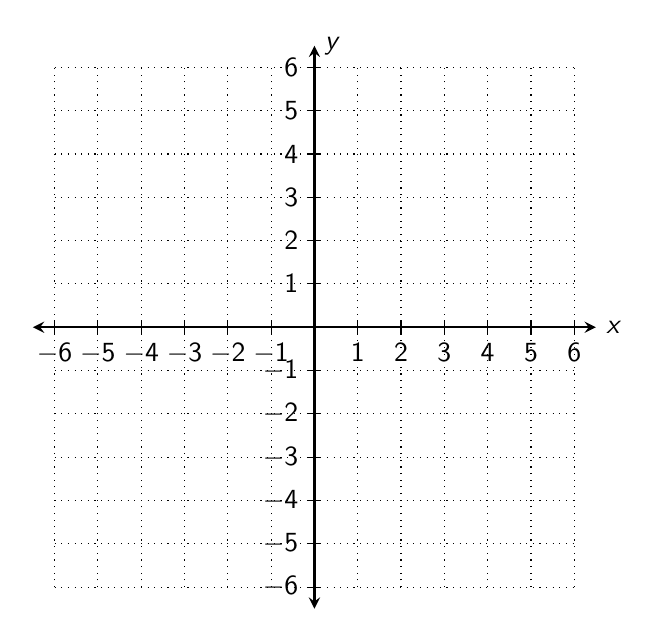
\begin{tikzpicture}[scale=0.55]
    \draw[<->, thick] (-6.5,0) -- (6.5,0) node [right] {$x$};
    \draw[<->, thick] (0,-6.5) -- (0,6.5) node [right] {$y$};
    \draw[dotted] (-6,-6) grid (6,6);
    \foreach \x in {-6,...,-1,,1,...,6}
    \draw (\x, 0.15) -- (\x,-0.15) node [below] {$\tiny \x$};
    \foreach \y in {-6,...,-1,,1,...,6}
    \draw (0.15,\y) -- (-0.15,\y) node [left] {$\tiny \y$};
\end{tikzpicture}
\end{example}

\vspace{0.75in}

\begin{tcolorbox}[colframe=black!20!white, opacitybacktitle=0.1, coltitle=black, title=\textbf{Side-Angle-Side (SAS) Shortcut}]
If 2 sides and the included angle of one triangle are congruent to 2 sides and the included angle of another, then the triangles are congruent.
\newline

\begin{minipage}{0.3\textwidth}
\begin{itemize}
    \item $\triangle ABC \cong \triangle DEF$
\end{itemize}
\end{minipage}
\begin{minipage}{0.6\textwidth}
\begin{tikzpicture}
\tkzDefPoints{0/0/A, 1/1.5/B, 2.5/-0.5/C}
\tkzDrawPolygon(A,B,C)
\tkzLabelPoints[left](A)
\tkzLabelPoints[above](B)
\tkzLabelPoints[right](C)
\tkzMarkSegment[mark = |](A,B)
\tkzMarkSegment[mark = ||](A,C)
\tkzMarkAngle[size=0.5](C,A,B)
\end{tikzpicture}
\hspace{0.25in}
\begin{tikzpicture}
\tkzDefPoints{0/0/D, 1/1.5/E, 2.5/-0.5/F}
\tkzDrawPolygon(D,E,F)
\tkzLabelPoints[left](D)
\tkzLabelPoints[above](E)
\tkzLabelPoints[right](F)
\tkzMarkSegment[mark = |](D,E)
\tkzMarkSegment[mark = ||](D,F)
\tkzMarkAngle[size=0.5](F,D,E)
\end{tikzpicture}
\end{minipage}
\end{tcolorbox}

\vspace{0.5in}

\begin{example}
What other information would you need to prove the triangles congruent by SAS?

\begin{multicols}{2}
\begin{enumerate}[(a)]
\item \mbox{} \newline 
    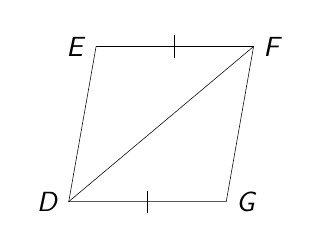
\begin{tikzpicture}
    \tkzDefPoints{0/0/D, 2/0/G}
    \tkzDefShiftPoint[D](80:2){E}
    \tkzDefShiftPoint[G](80:2){F}
    \tkzDrawPolygon(D,E,F,G)
    \tkzLabelPoints[left](D,E)
    \tkzLabelPoints[right](F,G)
    \tkzDrawSegment(D,F)
    \tkzMarkSegments[mark = |](D,G E,F)
    \end{tikzpicture}

\item \mbox{} \newline 
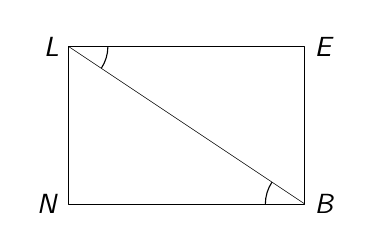
\begin{tikzpicture}
    \tkzDefPoints{0/0/N, 3/0/B, 3/2/E, 0/2/L}
    \tkzDrawPolygon(N,B,E,L)
    \tkzDrawSegment(L,B)
    \tkzLabelPoints[left](L,N)
    \tkzLabelPoints[right](B,E)
    \tkzMarkAngles[size=0.5](B,L,E L,B,N)
\end{tikzpicture}
\end{enumerate}
\end{multicols}
\end{example}

\newpage 

\begin{example}
Would you use SSS or SAS to prove the triangles congruent? If there isn't enough information to prove congruence, write \textit{not enough info}. Justify your answers.
\newline\\

\begin{tabular}{p{0.5\textwidth}p{0.5\textwidth}}
(a) &   (b) \\[0.1in]
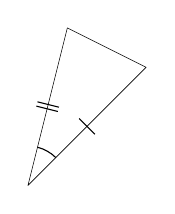
\begin{tikzpicture}
    \tkzDefPoints{0/0/A, 1/-0.5/B, -0.5/-2/C}
    \tkzDrawPolygon(A,B,C)
    \tkzMarkSegment[mark=|](B,C)
    \tkzMarkSegment[mark=||](A,C)
    \tkzMarkAngle[size=0.5](B,C,A)
\end{tikzpicture}
\hspace{0.25in}
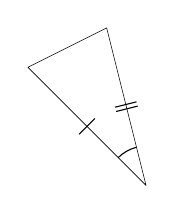
\begin{tikzpicture}
    \tkzDefPoints{0/0/A, -1/-0.5/B, 0.5/-2/C}
    \tkzDrawPolygon(A,B,C)
    \tkzMarkSegment[mark=|](B,C)
    \tkzMarkSegment[mark=||](A,C)
    \tkzMarkAngle[size=0.5](A,C,B)
\end{tikzpicture}
&
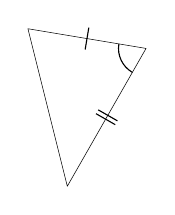
\begin{tikzpicture}
    \tkzDefPoints{0/0/A, 1.5/-0.25/B, 0.5/-2/C}
    \tkzDrawPolygon(A,B,C)
    \tkzMarkSegment[mark=|](A,B)
    \tkzMarkSegment[mark=||](B,C)
    \tkzMarkAngle[size=0.35](A,B,C)
\end{tikzpicture}
\hspace{0.25in}
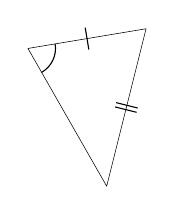
\begin{tikzpicture}
    \tkzDefPoints{0/0/A, -1.5/-0.25/B, -0.5/-2/C}
    \tkzDrawPolygon(A,B,C)
    \tkzMarkSegment[mark=|](A,B)
    \tkzMarkSegment[mark=||](A,C)
    \tkzMarkAngle[size=0.35](C,B,A)
\end{tikzpicture}
\\[1in]
(c) &   (d) \\[0.1in]
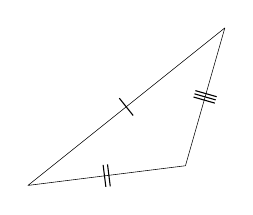
\begin{tikzpicture}
    \tkzDefPoints{0/0/A, 2/0.25/B, 2.5/2/C}
    \tkzDrawPolygon(A,B,C)
    \tkzMarkSegment[mark=|](A,C)
    \tkzMarkSegment[mark=||](A,B)
    \tkzMarkSegment[mark=|||](B,C)
\end{tikzpicture}
\hspace{0.25in}
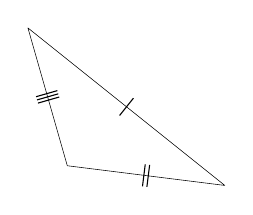
\begin{tikzpicture}
    \tkzDefPoints{0/0/A, -2/0.25/B, -2.5/2/C}
    \tkzDrawPolygon(A,B,C)
    \tkzMarkSegment[mark=|](A,C)
    \tkzMarkSegment[mark=||](A,B)
    \tkzMarkSegment[mark=|||](B,C)
\end{tikzpicture}
&
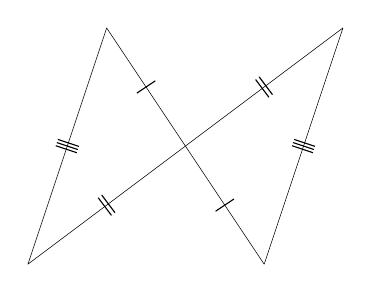
\begin{tikzpicture}
    \tkzDefPoints{0/0/A, 4/3/E, 2/1.5/C, 1/3/B, 3/0/D}
    \tkzDrawPolygon(A,B,D,E)
    \tkzMarkSegments[mark=|](C,B C,D)
    \tkzMarkSegments[mark=||](A,C C,E)
    \tkzMarkSegments[mark=|||](A,B D,E)
\end{tikzpicture}
\end{tabular}
\end{example}

\end{document}
